\section{Results}

% Results: you should assess the success of your project. How does it compare with the
% original specification? How reliable is it? How have you tested it? Comment on its
% robustness. This is done in the final documentation of the project.

We tested the Devault with uploading, downloading, sharing, deleting, connecting, and disconnecting functionality on different browsers and devices. Below we show the results of three of these tests. \\

\noindent
\textbf{1. \textit{Brave browser, the desktop version and metamask}} \\

Figure \ref{img:connectResult} shows the result of connecting the wallet.

\namedfigure
{!hbtp}
{img:connectResult}
{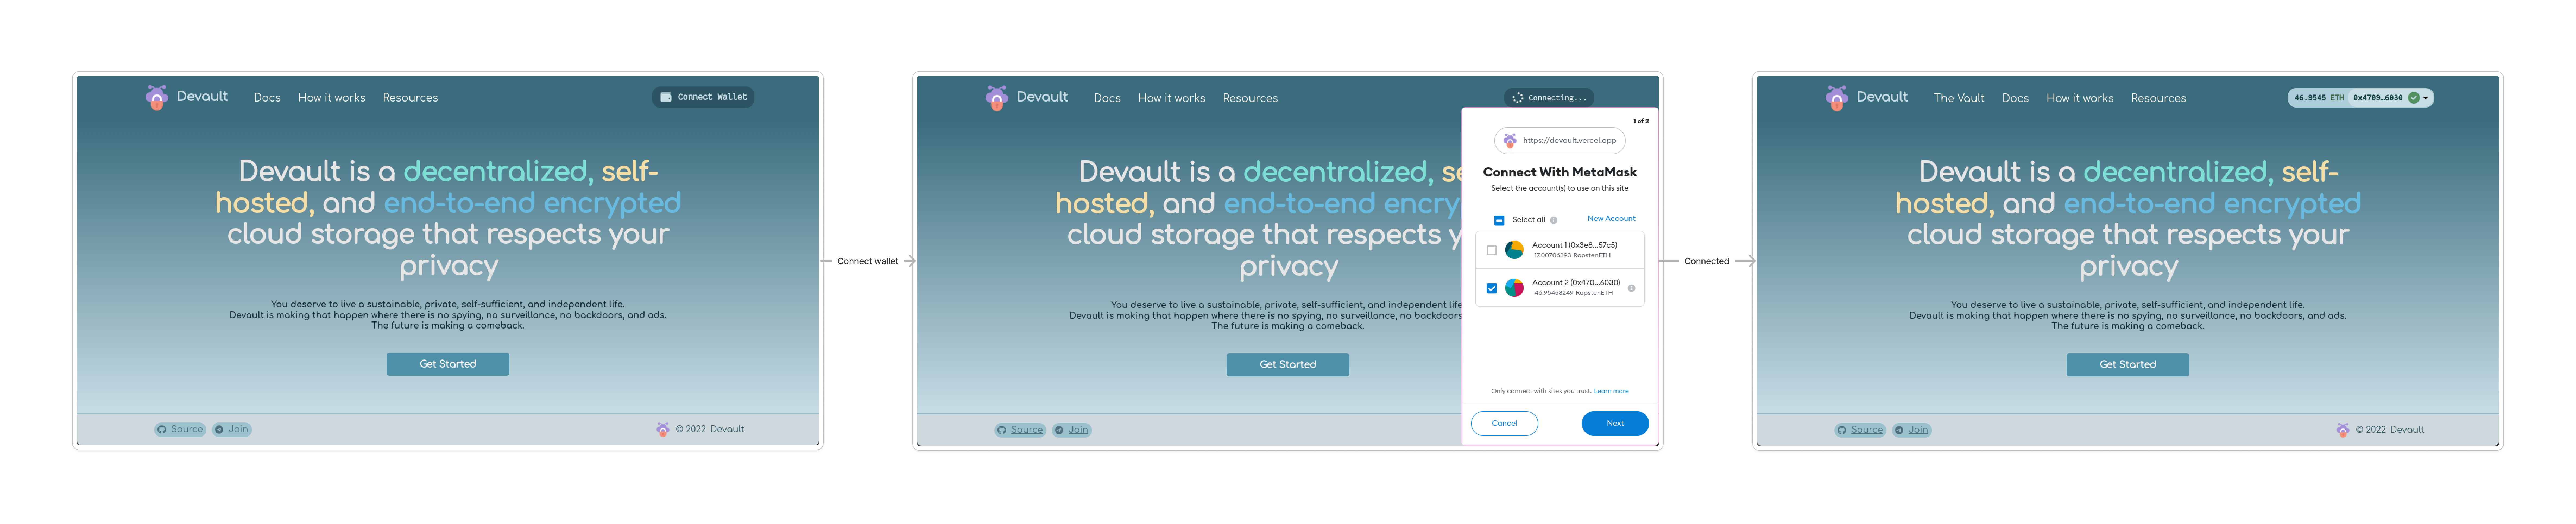
\includegraphics[width=\textwidth]{connect_result.png}}
{The user experience of connecting wallet.}


\newpage
\noindent
\textbf{2. \textit{Brave browser, the mobile version and brave wallet}} \\

Figure \ref{img:uploadResult} shows the result of uploading files functionality.

\namedfigure
{!hbtp}
{img:uploadResult}
{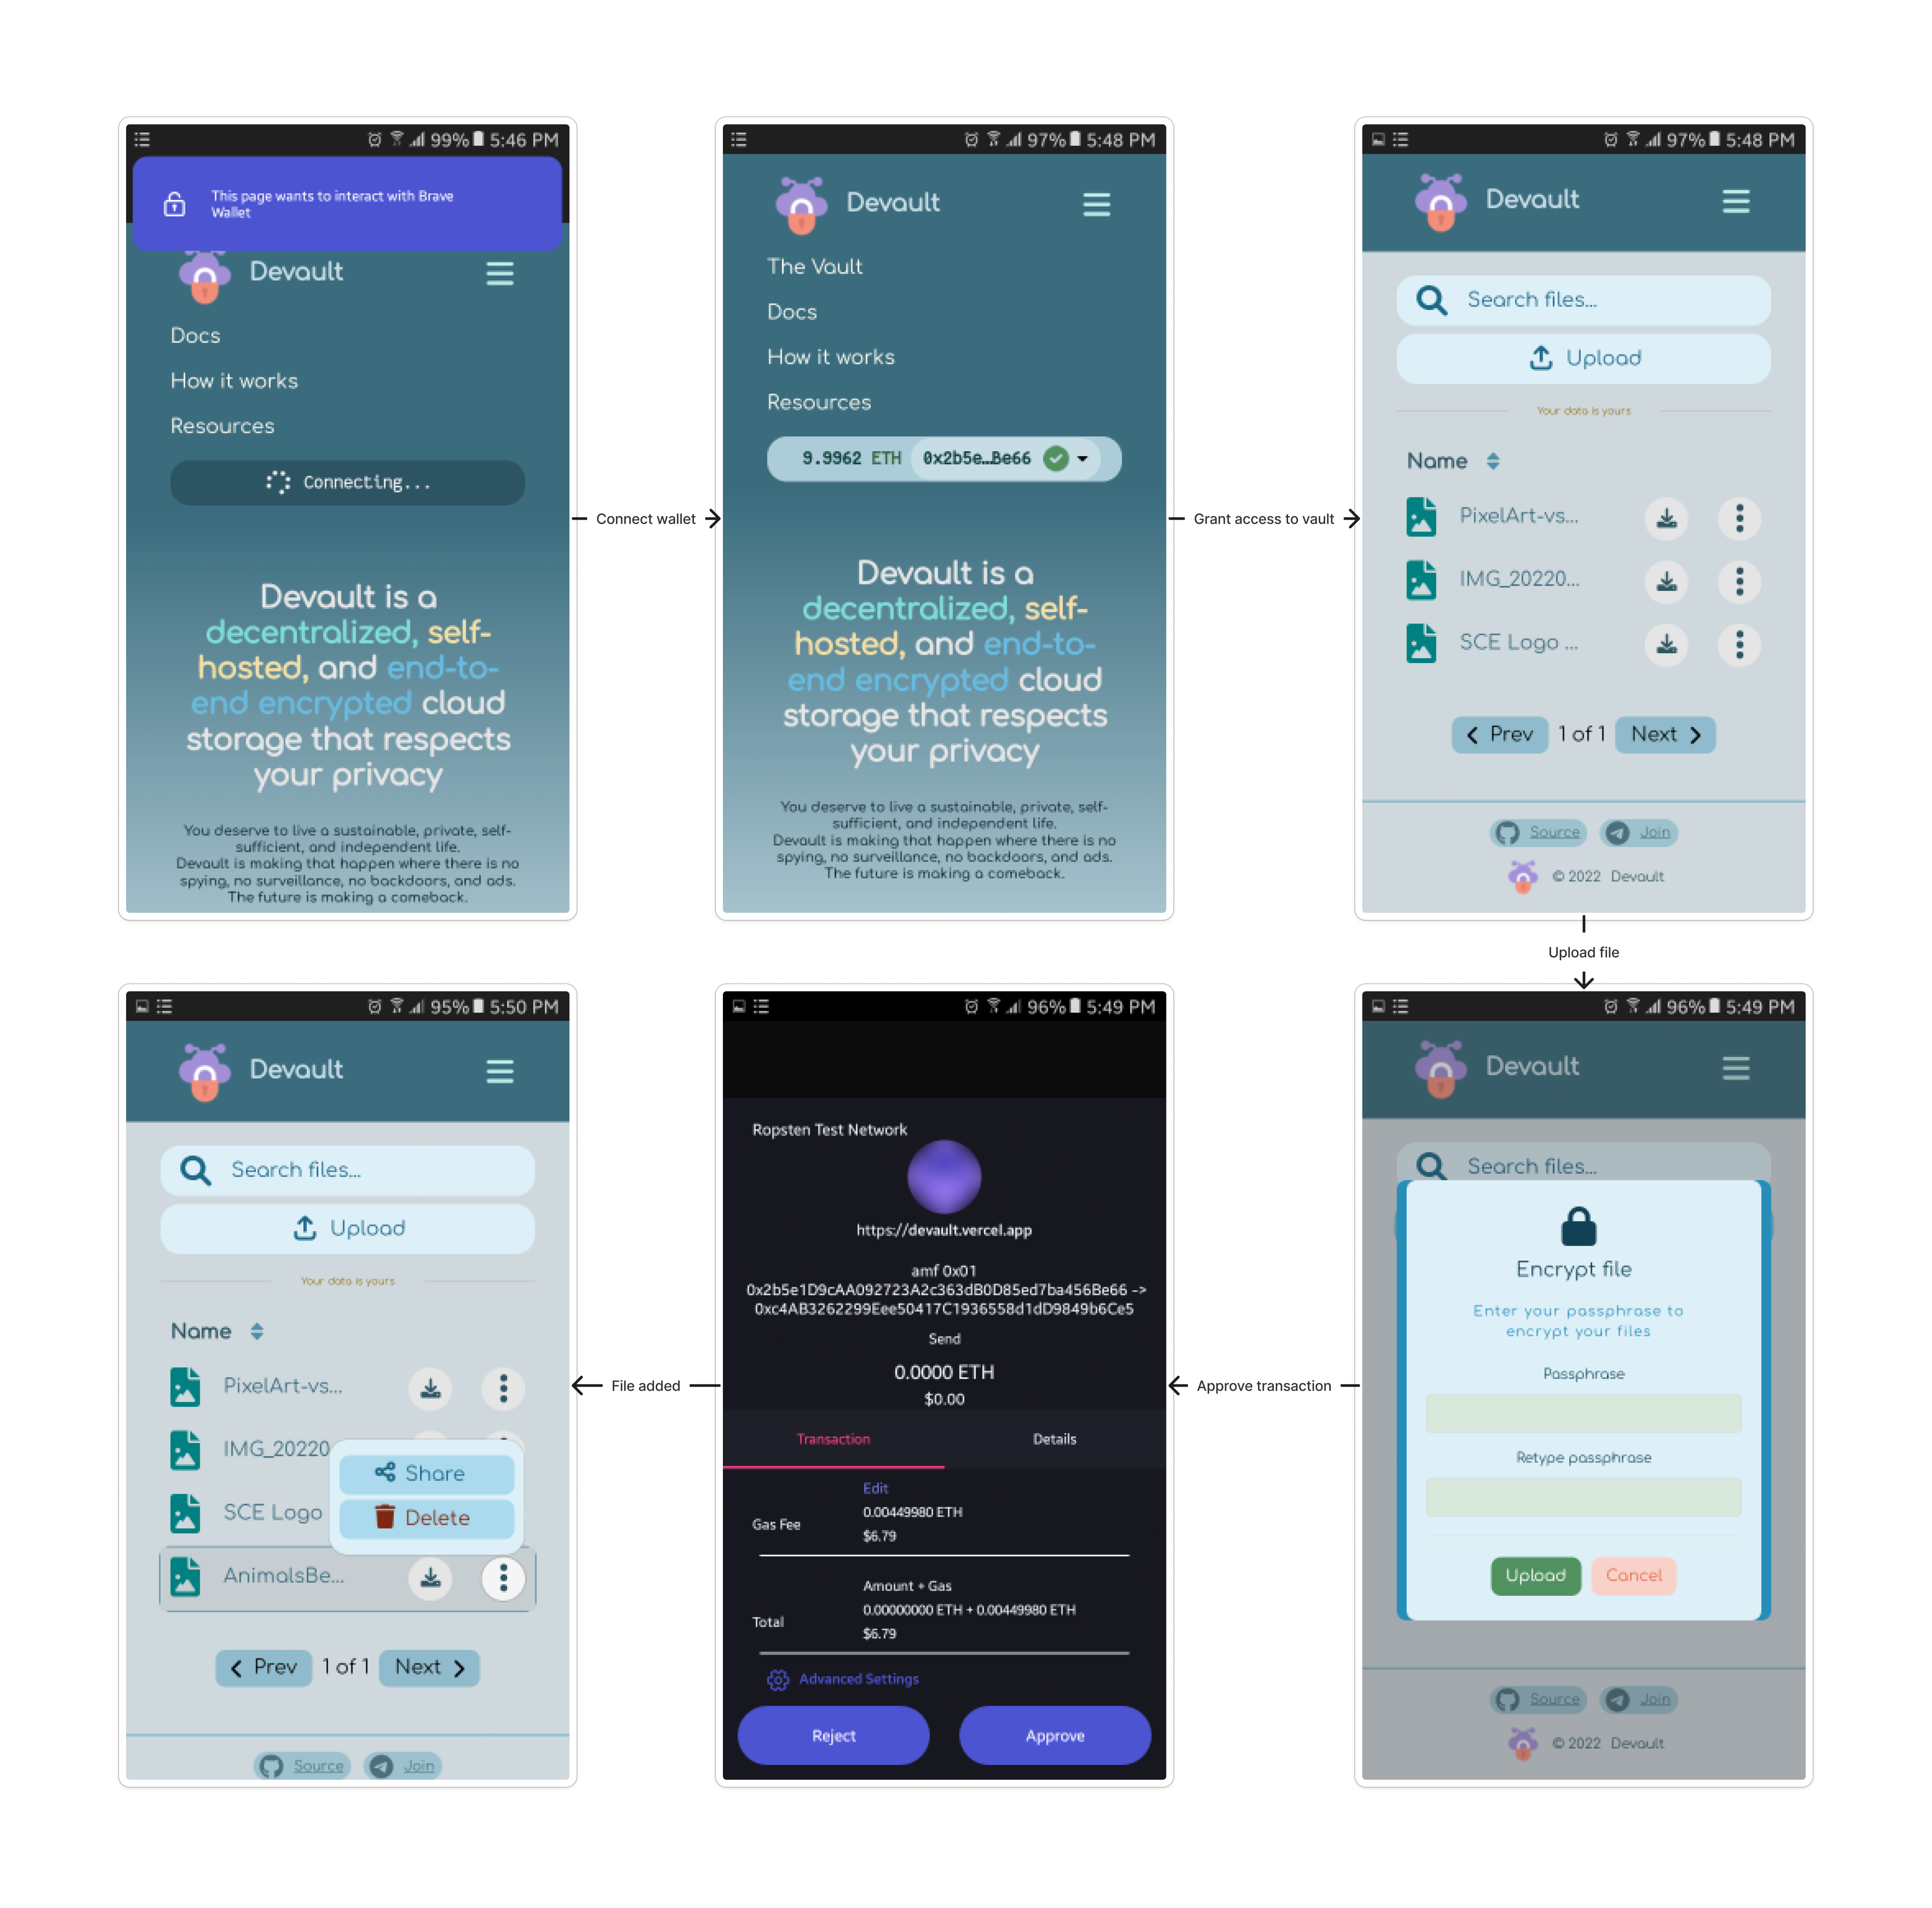
\includegraphics[width=\textwidth]{upload_result.pdf}}
{The user experience of uploading files.}


\newpage
\noindent
\textbf{3. \textit{Firefox browser, the desktop version and metamask}} \\

Figure \ref{img:shareResult} shows the result of sharing files functionality.

\namedfigure
{!hbtp}
{img:shareResult}
{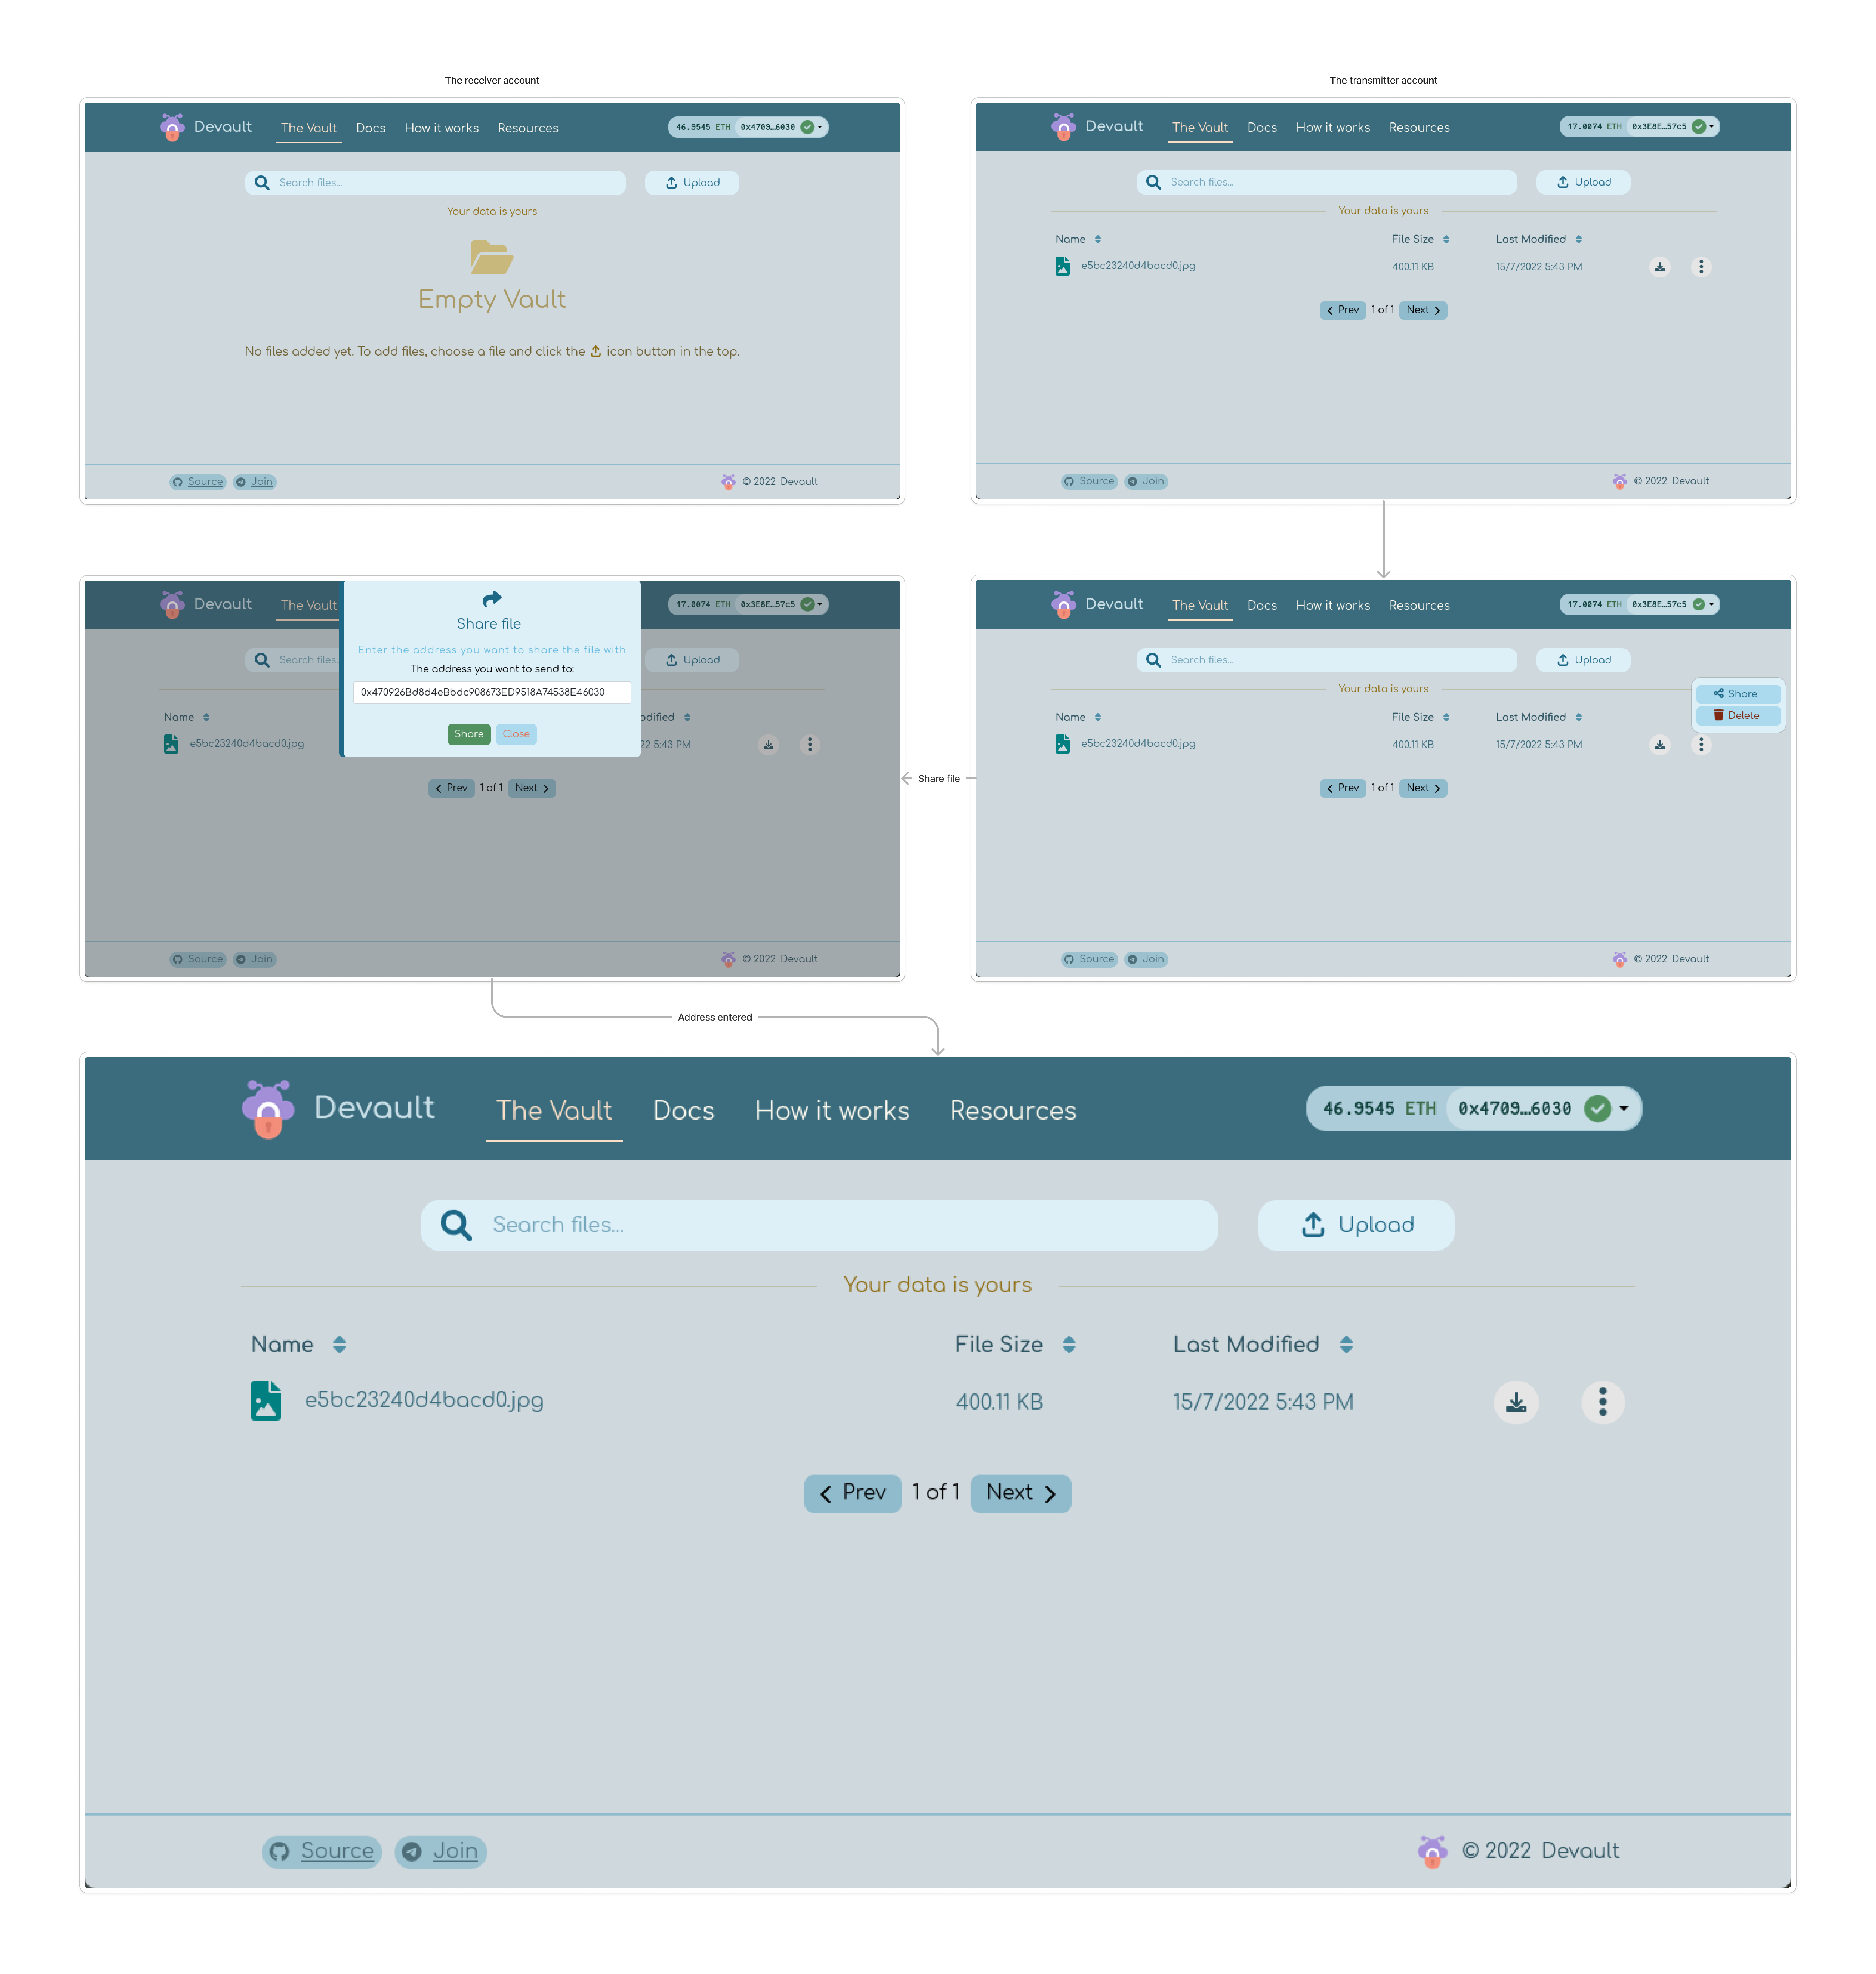
\includegraphics[width=\textwidth]{share_result.png}}
{The user experience of sharing files.}


\newpage
\subsection{Performance}

For performance testing we used GTmetrix tool.

GTmetrix is one of the most popular tools for analyzing site speed performance. If you put a website to the test, it will provide a performance score and a report which shows the current state of the site along with some suggestions on what can be improved.
Figure \ref{img:gtmetrixTest} shows performance of devault has reached the highest grade.

\namedfigure
{!htbp}
{img:gtmetrixTest}
{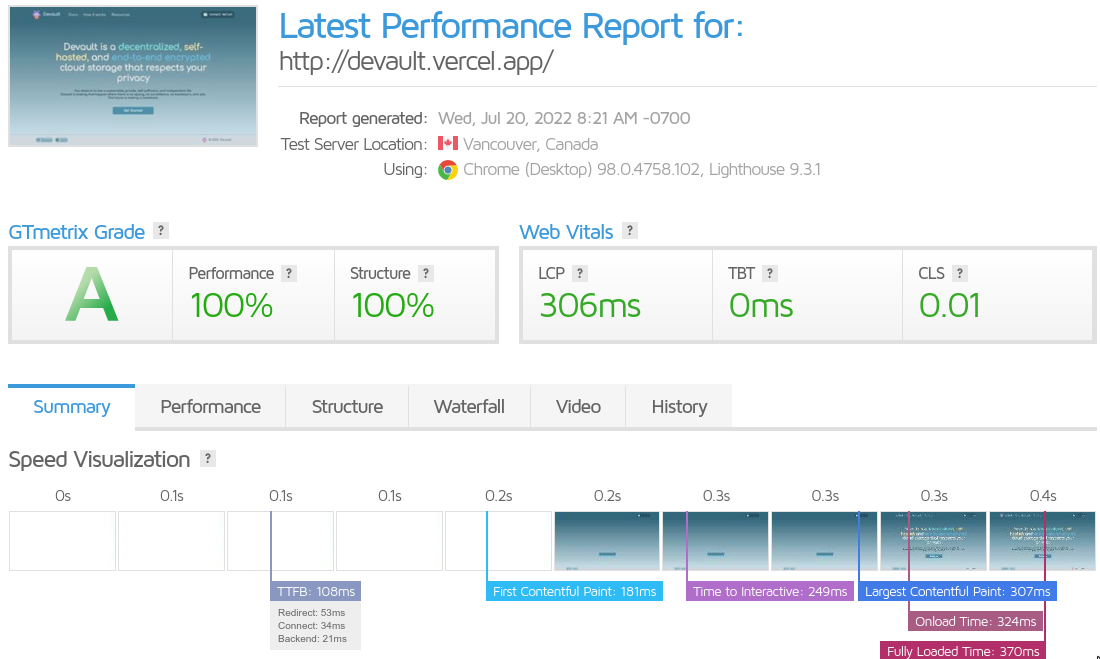
\includegraphics[width=\textwidth]{gtmetrix_test.png}}
{The performance report of devault generated by GTMetrix.}


\begin{table}[!ht]
  \centering
  \caption{The performance report details}
  \begin{tabular}{p{0.35\linewidth} p{0.35\linewidth}}
    \toprule
    Performance Metrics & The measure
    \\\midrule
    Total Page Size & 450KB. \\
    Total Page Requests & 31. \\
    Fully Loaded Time & 370ms. \\
    Largest Content Element & 306ms
    \\\bottomrule
  \end{tabular}
\end{table}